\section{程序的机器级表示:控制}
\subsection{条件码}
\subsubsection{处理器状态与条件码概述}
在 x86 - 64 架构中,处理器状态包含多个部分,存储当前程序的执行信息
\begin{enumerate}
    \item 临时数据,\mintinline{asm}{%rax} 等
    \item 运行时栈的位置(栈顶),\mintinline{asm}{%rsp}
    \item 当前代码控制点的位置(即将要执行的指令地址),\mintinline{asm}{%rip}
    \item 条件码,包括CF、ZF、SF、OF
\end{enumerate}
条件码寄存器是简单的位寄存器,通过算术运算、比较指令和测试指令等进行设置。

\subsubsection{条件码含义}
\begin{enumerate}
    \item CF: 进位标志 (Carry Flag)。最近的操作使无符号数最高位产生了进位,可用来检查无符号操作的溢出
    \item ZF: 零标志 (Zero Flag)。最近的操作得出的结果为 0
    \item SF: 符号标志 (Sign Flag)。最近的操作得到的结果为负数
    \item OF: 溢出标志 (Overflow Flag)。最近的操作导致一个有符号数补码溢出
\end{enumerate}


\subsubsection{条件码的设置方式}
\begin{enumerate}
    \item \textbf{算术运算隐式设置}: \mintinline{asm}{addq Src, Dest},相当于$t =a + b$

          这类算术运算指令会隐式设置条件码。若运算时出现无符号数运算溢出,CF 被置位;若 \(t == 0\),ZF 被置位;若有符号数 \(t < 0\)(,SF 被置位;若有符号数运算出现溢出,即 \mintinline{c}{(a > 0 && b > 0 && t < 0) || (a < 0 && b < 0 && t >= 0)},OF 被置位。需要注意的是,\mintinline{asm}{\leaq} 指令不修改条件码。
    \item \textbf{比较指令显式设置}:\mintinline{asm}{cmpq Src2, Src1}(如 \mintinline{asm}{cmpq b,a} )

          指令类似于计算 \(a - b\),但不将结果写入目标寄存器,而是根据计算结果显式设置条件码。当运算时出现超出最高位的借位(用于无符号数比较),CF 被置位;若 \(a == b\),ZF 被置位;若 \((a - b)<0\)(看做有符号数),SF 被置位;若有符号数运算出现溢出,即 \mintinline{c}{(a > 0 && b < 0 && (a - b) < 0) || ( a < 0 && b > 0 && (a - b) > 0)} ,OF 被置位。
    \item \textbf{测试指令显式设置}:\mintinline{asm}{testq Src2, Src1}(如 \mintinline{asm}{testq b,a} )

          指令类似于计算 \(a \& b\),同样不将结果写入目标寄存器,而是根据 \(a \& b\) 的结果设置条件码。常用于对一个操作数的某几个位进行掩码检测,当 \(a \& b == 0\) 时,ZF 被置位;若 \((a \& b)<0\),SF 被置位。
\end{enumerate}

\subsubsection{读取条件码与 SetX 指令}
SetX 指令可根据条件码表达式将目标寄存器的最后一个字节修改为 0 或 1,且不会影响目标寄存器最高 7 个字节的值。常见的 SetX 指令如下:
\begin{table}[H]
    \captionsetup{skip=4pt}
    \centering
    \setlength{\arrayrulewidth}{1pt}
    \begin{tabular}{ccc}
        \hline
        SetX 指令                 & 条件                           & 描述                   \\
        \hline
        \mintinline{asm}{sete}  & \mintinline{asm}{ZF}         & 相等/为零                \\
        \mintinline{asm}{setne} & \mintinline{asm}{~ZF}        & 不相等/不为零              \\
        \mintinline{asm}{sets}  & \mintinline{asm}{SF}         & 负数                   \\
        \mintinline{asm}{setns} & \mintinline{asm}{~SF}        & 非负数                  \\
        \mintinline{asm}{setg}  & \mintinline{asm}{~(SF^OF)    & ~ZF}       & 大于(有符号) \\
        \mintinline{asm}{setge} & \mintinline{asm}{~(SF^OF)}   & 大于或等于(有符号)           \\
        \mintinline{asm}{setl}  & \mintinline{asm}{(SF^OF)}    & 小于(有符号)              \\
        \mintinline{asm}{setle} & \mintinline{asm}{(SF^OF)|ZF} & 小于或等于(有符号)           \\
        \mintinline{asm}{seta}  & \mintinline{asm}{~CF & ~ZF}       & 高于(无符号) \\
        \mintinline{asm}{setb}  & \mintinline{asm}{CF}         & 低于(无符号)              \\
        \hline
    \end{tabular}
    \caption{SetX 指令与条件码关系}
\end{table}
以函数 \(\text{gt}\) 为例:
\begin{multicols}{2}
    \begin{minted}{c}
int gt(long x, long y){
    return x > y;
}
\end{minted}
    \columnbreak
    \begin{minted}{asm}
gt:
    cmpq    %rsi, %rdi     # Compare x:y
    setg    %al            # Set when >
    movzbl  %al, %eax      # Set rest of %rax zero 
    ret
\end{minted}
\end{multicols}
在 x86 - 64 指令集中,32 位操作指令会将目标寄存器的高 32 位清 0。

\subsection{条件分支}
\subsubsection{跳转指令(jX 指令)}
jX 指令根据条件码跳转到代码的其他位置执行,常见的 jX 指令如下:
\begin{table}[H]
    \captionsetup{skip=4pt}
    \centering
    \setlength{\arrayrulewidth}{1pt}
    \begin{tabular}{ccc}
        \hline
        jX 指令                 & 条件                              & 描述            \\
        \hline
        \mintinline{asm}{jmp} & 1                               & 无条件跳转         \\
        \mintinline{asm}{je}  & \mintinline{asm}{ZF}            & 相等/为零则跳转      \\
        \mintinline{asm}{jne} & \mintinline{asm}{~ZF}           & 不相等/不为零则跳转    \\
        \mintinline{asm}{js}  & \mintinline{asm}{SF}            & 负数则跳转         \\
        \mintinline{asm}{jns} & \mintinline{asm}{~SF}           & 非负数则跳转        \\
        \mintinline{asm}{jg}  & \mintinline{asm}{~(SF^OF)\&~ZF} & 大于(有符号)则跳转    \\
        \mintinline{asm}{jge} & \mintinline{asm}{~(SF^OF)}      & 大于或等于(有符号)则跳转 \\
        \mintinline{asm}{jl}  & \mintinline{asm}{(SF^OF)}       & 小于(有符号)则跳转    \\
        \mintinline{asm}{jle} & \mintinline{asm}{(SF^OF)|ZF}    & 小于或等于(有符号)则跳转 \\
        \mintinline{asm}{ja}  & \mintinline{asm}{~CF\&~ZF}      & 高于(无符号)则跳转    \\
        \mintinline{asm}{jb}  & \mintinline{asm}{CF}            & 低于(无符号)则跳转    \\
        \hline
    \end{tabular}
    \caption{jX 指令与条件码关系}
\end{table}

% \subsubsection{跳转指令的编码示例}
% 以一段简单的汇编代码为例:
% \begin{minted}{asm}
% loop:
%     movq    %rdi, %rax
%     jmp     .L2
% .L3:
%     sarq    %rax
% .L2:
%     testq   %rax, %rax
%     jg      .L3
%     rep; ret
% \end{minted}
% 对应的机器码如下:
% \begin{minted}{asm}
% 4004d0: 48 89 f8           movq %rdi, %rax
% 4004d3: eb 03              jmp 4004d8<loop+0x8>
% 4004d5: 48 d1 f8           sarq %rax
% 4004d8: 48 85 c0           testq %rax, %rax
% 4004db: 7f f8              jg 4004d5<loop+0x5>
% 4004dd: f3 c3              repz retq
% \end{minted}

\subsubsection{条件分支示例(早期模式)}
对于 C 语言函数:
\begin{multicols}{2}
    \begin{minted}{c}
long absdiff(long x, long y){
    long result;
    if (x > y)
        result = x - y;
    else
        result = y - x;
    return result;
}
\end{minted}
    \columnbreak
    \begin{minted}{c}
    // goto version
    long absdiff_j(long x, long y){
        long result;
        int ntest = x <= y;
        if (ntest)
            goto Else;
        result = x - y;
        goto Done;
        Else:
            result = y - x;
        Done:
            return result;
    }
    \end{minted}
\end{multicols}

使用 \mintinline{bash}{gcc –Og -S –fno-if-conversion control.c} 生成的汇编代码如下(\mintinline{asm}{%rdi}表示 x,\mintinline{asm}{%rsi}表示 y,\mintinline{asm}{%rax}表示return的值):
\begin{minted}{asm}
absdiff:
    cmpq    %rsi, %rdi      # x:y
    jle     .L4             # x <= y 跳转 L4
    movq    %rdi, %rax      # ret <- x
    subq    %rsi, %rax      # ret -= y
    ret
.L4:                        # x <= y
    movq    %rsi, %rax      # ret <- y
    subq    %rdi, %rax      # ret -= x
    ret
\end{minted}


\subsubsection{条件表达式的翻译(使用分支)}
对于条件表达式 \mintinline{c}{val = Test ? Then_Expr : Else_Expr;},可以使用 \mintinline{c}{goto} 语句版本实现:
\begin{minted}{c}
ntest = !Test;
if (ntest) goto Else;
val = Then_Expr;
goto Done;
Else:
    val = Else_Expr;
Done:
\end{minted}
这种方式为 \mintinline{c}{Then} 和 \mintinline{c}{Else} 表达式创建独立的代码块,根据条件选择合适的一个代码块并执行。

\subsubsection{条件数据移动指令}
在计算机处理器中,流水线技术允许最多有三条指令同时执行,提高了指令执行效率。然而,条件分支会破坏流水线的指令流,影响处理器性能。而条件数据移动指令不需要改变控制流,在某些情况下能避免这种性能损耗。

条件数据移动指令功能为 \mintinline{asm}{if (Test)  {Dest <- Src}} 。GCC 在编译时会尝试使用该指令翻译条件分支,但仅在保证逻辑安全的时候使用。以 \mintinline{c}{absdiff} 函数为例,使用条件数据移动指令的汇编代码如下:
\begin{minted}{asm}
absdiff:
    movq    %rdi, %rax      # x
    subq    %rsi, %rax      # result = x - y
    movq    %rsi, %rdx
    subq    %rdi, %rdx      # eval = y - x
    cmpq    %rsi, %rdi      # x:y
    cmovle  %rdx, %rax      # if x<=y, result = eval
    ret
\end{minted}
不过,在一些情况下不适合使用条件数据移动指令,比如存在大量计算、有风险的计算或有副作用的计算时。例如 \mintinline{c}{val = Test(x) ? Hard1(x) : Hard2(x);} 以及 \mintinline{c}{val = p ? *p : 0;} 还有 \mintinline{c}{val = x > 0 ? x*=7 : x+=3;} 等情况。

\subsection{循环}
\subsubsection{Do - While 循环示例与编译结果}
以计算无符号长整型数 \mintinline{c}{x} 编码中“1”的个数的函数为例:
\begin{minted}{c}
long pcount_do(unsigned long x){
    long result = 0;
    do {
        result += x & 0x1;
        x >>= 1;
    } while (x);
    return result;
}
\end{minted}
其使用 \mintinline{c}{goto} 语句等价表示为:
\begin{minted}{c}
long pcount_goto(unsigned long x){
    long result = 0;
    loop:
        result += x & 0x1;
        x >>= 1;
        if(x) goto loop;
        return result;
}
\end{minted}
编译后的汇编代码如下:
\begin{minted}{asm}
movl        $0, %eax    # result = 0
.L2:                    # loop:
    movq    %rdi, %rdx
    andl    $1, %edx    # t = x & 0x1
    addq    %rdx, %rax  # result += t
    shrq    %rdi        # x >>= 1
    jne     .L2         # if (x) goto loop
    rep; ret
\end{minted}
其中,\mintinline{asm}{\%rdi} 用于传递参数 \mintinline{c}{x},\mintinline{asm}{\%rax} 用于存储 \mintinline{c}{result} 。

\subsubsection{While 循环通用的翻译方式}
\begin{enumerate}
    \item \textbf{“跳转到中间”翻译方法(使用 \mintinline{bash}{–Og} 编译优化选项)}

          对于 \mintinline{c}{while (Test) Body} 结构,翻译为 \mintinline{c}{goto} 版本如下:
          \begin{minted}{c}
goto test;
loop:
    Body
test:
    if (Test)
    goto loop;
done:
\end{minted}
          以计算无符号长整型数 \mintinline{c}{x} 编码中“1”的个数的 \mintinline{c}{while} 循环函数为例:
          \begin{multicols}{2}
              \begin{minted}{c}
// while 版本
long pcount_while(unsigned long x){
    long result = 0;
    while (x) {
        result += x & 0x1;
        x >>= 1;
    }
    return result;
}
\end{minted}
              \columnbreak
              \begin{minted}{c}
// goto 版本
long pcount_goto_jtm(unsigned long x){
    long result = 0;
    goto test;
    loop:
        result += x & 0x1;
        x >>= 1;
    test:
        if(x) goto loop;
        return result;
}
\end{minted}
          \end{multicols}

          与 \mintinline{c}{do - while} 循环相比,该方式在循环开始前先跳转至循环条件检测的位置。
    \item \textbf{另一种翻译方法(使用 \mintinline{bash}{–O1} 编译优化选项)}

          对于 \mintinline{c}{while (Test) Body} 结构,翻译为 \mintinline{c}{goto} 版本为:
          \begin{minted}{c}
    if (!Test)
        goto done;
    loop:
        Body
    if (Test)
        goto loop;
    done:
\end{minted}
          以计算无符号长整型数 \mintinline{c}{x} 编码中“1”的个数的 \mintinline{c}{while} 循环函数为例,对应的此版本代码为:
          \begin{minted}{c}
long pcount_goto_dw(unsigned long x){
    long result = 0;
    if (!x) goto done;
    loop:
        result += x & 0x1;
        x >>= 1;
        if(x) goto loop;
    done:
        return result;
}
\end{minted}
          与 \mintinline{c}{do - while} 循环相比,这种方式在循环开始前先检测循环条件,再进入循环。
\end{enumerate}

\subsubsection{For 循环一般形式与转换}
For 循环的一般形式为 \mintinline{c}{for (Init; Test; Update) Body},可以转换为 \mintinline{c}{while} 循环和 \mintinline{c}{goto} 版本。例如:
\begin{multicols}{2}
    \begin{minted}{c}
#define WSIZE 8 * sizeof(int)
long pcount_for(unsigned long x){
    size_t i;
    long result = 0;
    for (i = 0; i < WSIZE; i++) {
        unsigned bit = (x >> i) & 0x1;
        result += bit;
    }
    return result;
}
\end{minted}
\columnbreak
\begin{minted}{c}
    // goto version
    long pcount_for_gt(unsigned x) {
        int i;
        int result = 0;
        i = 0;
        if (!(i < WSIZE)) goto done;  //可以被编译器优化
        loop:
        unsigned bit = (x >> i) & 0x1;
        result += bit;
        i++;
        if (i < WSIZE)
            goto loop;
        done:
        return result;
    }
    \end{minted}
\end{multicols}

转换为 \mintinline{c}{while} 循环如下:
\begin{minted}{c}
long pcount_for_while(unsigned long x){
    size_t i;
    long result = 0;
    i = 0;
    while (i < WSIZE)
    {
        unsigned bit = (x >> i) & 0x1;
        result += bit;
        i++;
    }
    return result;
}
\end{minted}

\subsection{switch语句}
\subsubsection{switch的一般形式及跳转表}

\mintinline{c}{switch} 语句的一般形式如下:
\begin{minted}{c}
switch(x) {
    case val_0:
        Block 0;
    case val_1:
        Block 1;
      ......
    case val_(n-1):
        Block n-1;
}
    \end{minted}
对应的跳转表结构为:
\begin{figure}[H]
    \centering
    \captionsetup{skip=4pt}
    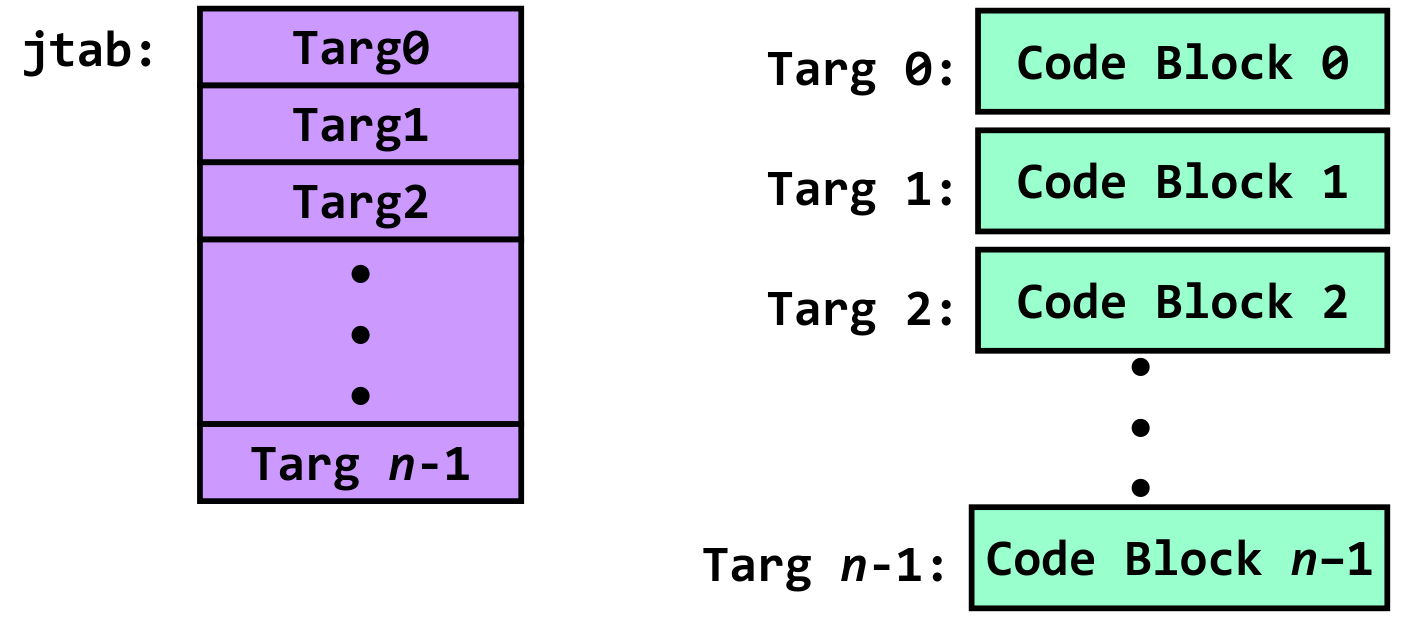
\includegraphics[width=10cm]{8.png}
    \caption{跳转表}
\end{figure}
翻译后(扩展 C)的形式为 \mintinline{c}{goto *JTab[op];},可通过跳转表快速根据 \mintinline{c}{x} 的值跳转到相应的代码块执行。


\subsubsection{分析跳转表}
以 \mintinline{c}{switch_eg} 函数为例:
\begin{minted}{c}
long switch_eg(long x, long y, long z) {
    long w = 1;
    switch(x) {
        ...
    }
    return w;
}
\end{minted}
其汇编代码如下:
\begin{minted}{asm}
setup: 
switch_eg:   
    movq    %rdx, %rcx 
    cmpq    $6, %rdi        # x:6 
    ja      .L8             # Use default if x > 6
    jmp     *.L4(,%rdi,8)   # goto *JTab[x] 
\end{minted}
其中,\mintinline{asm}{jmp *.L4(,%rdi,8)} 表示间接跳转到由 \mintinline{asm}{.L4} 开始的跳转表中索引为 \mintinline{c}{x}(\mintinline{asm}{%rdi} 存储 \mintinline{c}{x} 的值)的位置。当 \mintinline{c}{x} 大于 \mintinline{asm}{6} 时,会跳转到 \mintinline{asm}{.L8} 执行默认情况。注意,\mintinline{c}{w} 并没有在 \mintinline{c}{switch} 开始前初始化。

跳转表在汇编代码中的定义如下:
\begin{minted}{asm}
.section .rodata    # read-only data
    .align 8
.L4:
    .quad   .L8     # x = 0
    .quad   .L3     # x = 1
    .quad   .L5     # x = 2
    .quad   .L9     # x = 3
    .quad   .L8     # x = 4
    .quad   .L7     # x = 5
    .quad   .L7     # x = 6
\end{minted}
跳转表的基地址是 \mintinline{asm}{.L4},每个跳转目标需要 8 个字节(因为在 64 位系统中,地址是 8 个字节)。间接跳转时,缩放因子必须是 8 的整倍数,通过计算地址 \mintinline{asm}{.L4 + x * 8} 来获得跳转目标的位置(仅限于 \mintinline{asm}{0 <= x <= 6} 的情况)。

\subsubsection{代码块实现}
\begin{enumerate}
    \item \textbf{代码块(\mintinline{asm}{x == 1})}
          \begin{multicols}{2}
              \begin{minted}{asm}
.L3:
    movq    %rsi, %rax # y
    imulq   %rdx, %rax # y*z
    ret
    \end{minted}
              \columnbreak
              \begin{minted}{c}
        case 1:
            w = y*z;
            break;
    \end{minted}
          \end{multicols}
          当 \mintinline{c}{x} 等于 \mintinline{asm}{1} 时,执行此代码块,实现 \mintinline{c}{w = y*z} 的操作,其中 \mintinline{asm}{%rdi} 为参数 \mintinline{c}{x},\mintinline{asm}{%rsi} 为参数 \mintinline{c}{y},\mintinline{asm}{%rdx} 为参数 \mintinline{c}{z},\mintinline{asm}{%rax} 用于存储返回值。
    \item \textbf{处理落入另一个case的情况(\mintinline{asm}{x == 2,x == 3} )}
          \begin{multicols}{2}
              \begin{minted}{asm}
.L5:                    #Case2 
    movq    %rsi, %rax
    cqto
    idivq   %rcx        # y/z
    jmp     .L6         # goto merge 
.L9:                    # Case 3
    movl    $1, %eax    # w = 1
.L6:                    # merge:
    addq    %rcx, %rax  # w += z
    ret
    \end{minted}
              \columnbreak
              \begin{minted}{c}
        case 2:
            w = y/z;
            /* Fall Through */
        case 3:
            w += z;
            break;
    \end{minted}
          \end{multicols}

          对于 \mintinline{c}{case 2} 和 \mintinline{c}{case 3},\mintinline{c}{case 2} 执行完 \mintinline{c}{w = y/z} 后会继续执行 \mintinline{c}{case 3} 的代码,即跳转到 \mintinline{asm}{merge} 标签处执行 \mintinline{c}{w += z}。
    \item \textbf{代码块(\mintinline{c}{x == 5,x == 6} ,缺省)}
          \begin{multicols}{2}
              \begin{minted}{asm}
.L7:                    # Case 5,6
    movl    $1, %eax    # w = 1
    subq    %rdx, %rax  # w -= z
    ret
.L8:                    # Default:
    movl    $2, %eax    # 2
    ret
    \end{minted}
              \columnbreak
              \begin{minted}{c}
        case 5:
        case 6:
            w -= z;
            break;
        default:
            w = 2;
    \end{minted}
          \end{multicols}

          当 \mintinline{c}{x} 等于 \mintinline{asm}{5} 或 \mintinline{asm}{6} 时,执行 \mintinline{c}{w -= z};当 \mintinline{c}{x} 不满足任何 \mintinline{c}{case} 条件(即默认情况)时,执行 \mintinline{c}{w = 2}。
\end{enumerate}

\subsubsection{特殊情况处理}
\begin{enumerate}
    \item \textbf{没有从0处开始的情况}

          对于 \mintinline{c}{switch} 语句中 \mintinline{c}{case} 值不是从 \mintinline{asm}{0} 开始的情况,如:
          \begin{minted}{c}
void switch_eg_2(long x) {
    switch(x) {
        case 10000:
        ......
        case 10002:
        ......
        case 10005:
        ......
        default:
        ......
    }
}
    \end{minted}
          汇编代码会进行相应调整:
          \begin{minted}{asm}
switch_eg_2:
    leaq    -$10000(%rdi), %rsi     # %rsi = %rdi – 10000
    cmpq    $6, %rsi                # x:6
    ja      .L8                     # Use default
    jmp     *.L4(,%rsi,8)           # goto *JTab[x]
    \end{minted}
          通过 \mintinline{asm}{leaq -$10000(%rdi), %rsi} 将 \mintinline{c}{x} 的值进行调整,使其可以适配从 \mintinline{asm}{0} 开始索引的跳转表。
    \item \textbf{稀疏的switch语句}

          当 \mintinline{c}{switch} 语句的 \mintinline{c}{case} 值分布非常稀疏时,如:
          \begin{minted}{c}
switch(x) {
    case 0: 
            ...
    case 1000:
            ...
    case 92027:
            ...
}
    \end{minted}
          编译器可能会将其翻译为二分查找的语句(时间复杂度为 $O(\log n)$),而不是退化为逐个比较的 \mintinline{c}{if - else - if - else ...} 形式(时间复杂度为 $O(n)$),从而提高效率。
\end{enumerate}

\subsubsection{总结}
\mintinline{c}{switch} 语句通过条件跳转、间接跳转(利用跳转表实现)等机制实现其功能。编译器会根据 \mintinline{c}{switch} 语句的具体情况,如 \mintinline{c}{case} 值的连续性、数量等,自动生成合适的代码序列,以实现更复杂的控制逻辑。大规模的 \mintinline{c}{switch} 语句通常使用跳转表实现,而稀疏的 \mintinline{c}{switch} 语句则可以使用决策树(二分查找)来优化实现。
